% Options for packages loaded elsewhere
\PassOptionsToPackage{unicode}{hyperref}
\PassOptionsToPackage{hyphens}{url}
%
\documentclass[
]{article}
\title{ZipF}
\author{Marisangila Alves}
\date{27 April, 2022}

\usepackage{amsmath,amssymb}
\usepackage{lmodern}
\usepackage{iftex}
\ifPDFTeX
  \usepackage[T1]{fontenc}
  \usepackage[utf8]{inputenc}
  \usepackage{textcomp} % provide euro and other symbols
\else % if luatex or xetex
  \usepackage{unicode-math}
  \defaultfontfeatures{Scale=MatchLowercase}
  \defaultfontfeatures[\rmfamily]{Ligatures=TeX,Scale=1}
\fi
% Use upquote if available, for straight quotes in verbatim environments
\IfFileExists{upquote.sty}{\usepackage{upquote}}{}
\IfFileExists{microtype.sty}{% use microtype if available
  \usepackage[]{microtype}
  \UseMicrotypeSet[protrusion]{basicmath} % disable protrusion for tt fonts
}{}
\makeatletter
\@ifundefined{KOMAClassName}{% if non-KOMA class
  \IfFileExists{parskip.sty}{%
    \usepackage{parskip}
  }{% else
    \setlength{\parindent}{0pt}
    \setlength{\parskip}{6pt plus 2pt minus 1pt}}
}{% if KOMA class
  \KOMAoptions{parskip=half}}
\makeatother
\usepackage{xcolor}
\IfFileExists{xurl.sty}{\usepackage{xurl}}{} % add URL line breaks if available
\IfFileExists{bookmark.sty}{\usepackage{bookmark}}{\usepackage{hyperref}}
\hypersetup{
  pdftitle={ZipF},
  pdfauthor={Marisangila Alves},
  hidelinks,
  pdfcreator={LaTeX via pandoc}}
\urlstyle{same} % disable monospaced font for URLs
\usepackage[margin=1in]{geometry}
\usepackage{color}
\usepackage{fancyvrb}
\newcommand{\VerbBar}{|}
\newcommand{\VERB}{\Verb[commandchars=\\\{\}]}
\DefineVerbatimEnvironment{Highlighting}{Verbatim}{commandchars=\\\{\}}
% Add ',fontsize=\small' for more characters per line
\usepackage{framed}
\definecolor{shadecolor}{RGB}{248,248,248}
\newenvironment{Shaded}{\begin{snugshade}}{\end{snugshade}}
\newcommand{\AlertTok}[1]{\textcolor[rgb]{0.94,0.16,0.16}{#1}}
\newcommand{\AnnotationTok}[1]{\textcolor[rgb]{0.56,0.35,0.01}{\textbf{\textit{#1}}}}
\newcommand{\AttributeTok}[1]{\textcolor[rgb]{0.77,0.63,0.00}{#1}}
\newcommand{\BaseNTok}[1]{\textcolor[rgb]{0.00,0.00,0.81}{#1}}
\newcommand{\BuiltInTok}[1]{#1}
\newcommand{\CharTok}[1]{\textcolor[rgb]{0.31,0.60,0.02}{#1}}
\newcommand{\CommentTok}[1]{\textcolor[rgb]{0.56,0.35,0.01}{\textit{#1}}}
\newcommand{\CommentVarTok}[1]{\textcolor[rgb]{0.56,0.35,0.01}{\textbf{\textit{#1}}}}
\newcommand{\ConstantTok}[1]{\textcolor[rgb]{0.00,0.00,0.00}{#1}}
\newcommand{\ControlFlowTok}[1]{\textcolor[rgb]{0.13,0.29,0.53}{\textbf{#1}}}
\newcommand{\DataTypeTok}[1]{\textcolor[rgb]{0.13,0.29,0.53}{#1}}
\newcommand{\DecValTok}[1]{\textcolor[rgb]{0.00,0.00,0.81}{#1}}
\newcommand{\DocumentationTok}[1]{\textcolor[rgb]{0.56,0.35,0.01}{\textbf{\textit{#1}}}}
\newcommand{\ErrorTok}[1]{\textcolor[rgb]{0.64,0.00,0.00}{\textbf{#1}}}
\newcommand{\ExtensionTok}[1]{#1}
\newcommand{\FloatTok}[1]{\textcolor[rgb]{0.00,0.00,0.81}{#1}}
\newcommand{\FunctionTok}[1]{\textcolor[rgb]{0.00,0.00,0.00}{#1}}
\newcommand{\ImportTok}[1]{#1}
\newcommand{\InformationTok}[1]{\textcolor[rgb]{0.56,0.35,0.01}{\textbf{\textit{#1}}}}
\newcommand{\KeywordTok}[1]{\textcolor[rgb]{0.13,0.29,0.53}{\textbf{#1}}}
\newcommand{\NormalTok}[1]{#1}
\newcommand{\OperatorTok}[1]{\textcolor[rgb]{0.81,0.36,0.00}{\textbf{#1}}}
\newcommand{\OtherTok}[1]{\textcolor[rgb]{0.56,0.35,0.01}{#1}}
\newcommand{\PreprocessorTok}[1]{\textcolor[rgb]{0.56,0.35,0.01}{\textit{#1}}}
\newcommand{\RegionMarkerTok}[1]{#1}
\newcommand{\SpecialCharTok}[1]{\textcolor[rgb]{0.00,0.00,0.00}{#1}}
\newcommand{\SpecialStringTok}[1]{\textcolor[rgb]{0.31,0.60,0.02}{#1}}
\newcommand{\StringTok}[1]{\textcolor[rgb]{0.31,0.60,0.02}{#1}}
\newcommand{\VariableTok}[1]{\textcolor[rgb]{0.00,0.00,0.00}{#1}}
\newcommand{\VerbatimStringTok}[1]{\textcolor[rgb]{0.31,0.60,0.02}{#1}}
\newcommand{\WarningTok}[1]{\textcolor[rgb]{0.56,0.35,0.01}{\textbf{\textit{#1}}}}
\usepackage{graphicx}
\makeatletter
\def\maxwidth{\ifdim\Gin@nat@width>\linewidth\linewidth\else\Gin@nat@width\fi}
\def\maxheight{\ifdim\Gin@nat@height>\textheight\textheight\else\Gin@nat@height\fi}
\makeatother
% Scale images if necessary, so that they will not overflow the page
% margins by default, and it is still possible to overwrite the defaults
% using explicit options in \includegraphics[width, height, ...]{}
\setkeys{Gin}{width=\maxwidth,height=\maxheight,keepaspectratio}
% Set default figure placement to htbp
\makeatletter
\def\fps@figure{htbp}
\makeatother
\setlength{\emergencystretch}{3em} % prevent overfull lines
\providecommand{\tightlist}{%
  \setlength{\itemsep}{0pt}\setlength{\parskip}{0pt}}
\setcounter{secnumdepth}{-\maxdimen} % remove section numbering
\ifLuaTeX
  \usepackage{selnolig}  % disable illegal ligatures
\fi

\begin{document}
\maketitle

\hypertarget{paruxe2metros}{%
\subsubsection{Parâmetros}\label{paruxe2metros}}

\begin{verbatim}
Parâmetros      | Valores
----------------------|----------
alfa zipf             | 0.4, 0.6, 0.8, 1, 1.2 
lambda                | 5
n                     | 100
beta                  | 0.2
BS                    | 32
Cache                 | 100
UE                    | 200
Storage               | MBS 20GB SBS 4GB
Coverage              | MBS 300 SBS 70
RTT inicial           | CS/MBS 0.001s(1ms) MBS/MBS 0.001s(1ms) MBS/SBS 0.001s(1ms) SBS/UE 0.001s(1ms)
Tempo da Requisição   | 10 eventos
Mobilidade            | 10m
\end{verbatim}

\hypertarget{informauxe7uxf5es-da-aplicauxe7uxe3o.}{%
\subsubsection{Informações da
Aplicação.}\label{informauxe7uxf5es-da-aplicauxe7uxe3o.}}

\begin{verbatim}
Vazão Mínima |     Tamanho da Cache        | Buffer |
-------------|-----------------------------|--------|
100 Mbps    |      2GB/2000MB             |  48Mb  |
100 Mbps    |      4GB/4000MB             |  48Mb  |
100 Mbps    |      8GB/8000MB             |  48Mb  |
\end{verbatim}

\hypertarget{distribuiuxe7uxe3o-de-popularidade-do-conteuxfado-solicitado.}{%
\subsubsection{Distribuição de popularidade do conteúdo
solicitado.}\label{distribuiuxe7uxe3o-de-popularidade-do-conteuxfado-solicitado.}}

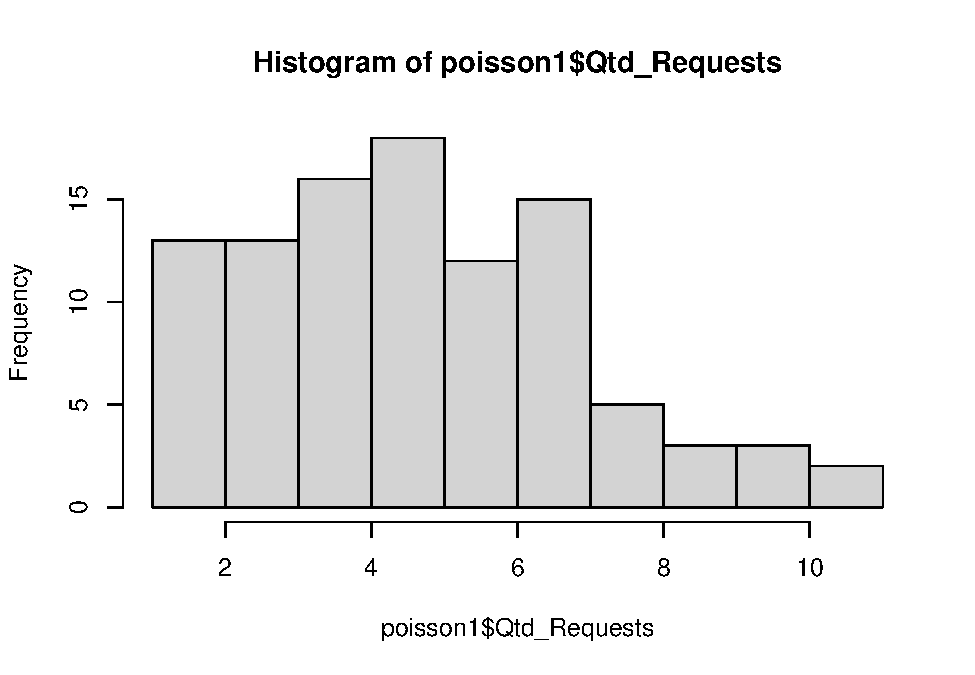
\includegraphics{analise_zipf2_files/figure-latex/unnamed-chunk-3-1.pdf}

\hypertarget{cache-cloud-e-storage.}{%
\subsubsection{Cache, Cloud e Storage.}\label{cache-cloud-e-storage.}}

\begin{verbatim}
## Saving 6.5 x 4.5 in image
## Saving 6.5 x 4.5 in image
## Saving 6.5 x 4.5 in image
## Saving 6.5 x 4.5 in image
## Saving 6.5 x 4.5 in image
## Saving 6.5 x 4.5 in image
\end{verbatim}

\includegraphics{analise_zipf2_files/figure-latex/unnamed-chunk-31-1.pdf}
\includegraphics{analise_zipf2_files/figure-latex/unnamed-chunk-31-2.pdf}
\includegraphics{analise_zipf2_files/figure-latex/unnamed-chunk-31-3.pdf}

\includegraphics{analise_zipf2_files/figure-latex/unnamed-chunk-41-1.pdf}

\begin{verbatim}
## Saving 6.5 x 4.5 in image
## Saving 6.5 x 4.5 in image
\end{verbatim}

\hypertarget{correlauxe7uxe3o-entre-proporuxe7uxf5es-e-variauxe7uxe3o-de-alpha}{%
\subsubsection{\texorpdfstring{Correlação entre proporções e variação de
\(\alpha\)}{Correlação entre proporções e variação de \textbackslash alpha}}\label{correlauxe7uxe3o-entre-proporuxe7uxf5es-e-variauxe7uxe3o-de-alpha}}

\begin{verbatim}
## [1] "Storage Load"
\end{verbatim}

\begin{verbatim}
## [1] -0.7028
\end{verbatim}

\begin{verbatim}
## [1] "Cache Hit"
\end{verbatim}

\begin{verbatim}
## [1] 0.648007
\end{verbatim}

\begin{verbatim}
## [1] "Cache Miss"
\end{verbatim}

\begin{verbatim}
## [1] -0.648007
\end{verbatim}

\hypertarget{correlauxe7uxe3o-entre-a-latuxeancia-e-variauxe7uxe3o-de-alpha}{%
\subsubsection{\texorpdfstring{Correlação entre a latência e variação de
\(\alpha\)}{Correlação entre a latência e variação de \textbackslash alpha}}\label{correlauxe7uxe3o-entre-a-latuxeancia-e-variauxe7uxe3o-de-alpha}}

\begin{verbatim}
## [1] 0.1454019
\end{verbatim}

\hypertarget{muxe9dias}{%
\subsubsection{Médias}\label{muxe9dias}}

\begin{verbatim}
##    Min. 1st Qu.  Median    Mean 3rd Qu.    Max. 
##   1.000   1.200   1.800   2.802   5.000   9.371
\end{verbatim}

\begin{verbatim}
##    0%   25%   50%   75%  100% 
## 1.000 1.200 1.800 5.000 9.371
\end{verbatim}

\begin{verbatim}
##   95% 
## 5.943
\end{verbatim}

\begin{verbatim}
##    Min. 1st Qu.  Median    Mean 3rd Qu.    Max. 
##   1.000   1.264   1.857   2.951   5.000   9.900
\end{verbatim}

\begin{verbatim}
##    0%   25%   50%   75%  100% 
## 1.000 1.264 1.857 5.000 9.900
\end{verbatim}

\begin{verbatim}
## 95% 
##   7
\end{verbatim}

\begin{verbatim}
##    Min. 1st Qu.  Median    Mean 3rd Qu.    Max. 
##   1.000   1.429   3.229   3.564   5.314  67.000
\end{verbatim}

\begin{verbatim}
##     0%    25%    50%    75%   100% 
##  1.000  1.429  3.229  5.314 67.000
\end{verbatim}

\begin{verbatim}
##   95% 
## 7.214
\end{verbatim}

\hypertarget{muxe1ximos}{%
\subsubsection{Máximos}\label{muxe1ximos}}

\begin{verbatim}
## [1] 0.18
\end{verbatim}

\begin{verbatim}
## [1] 0.82
\end{verbatim}

\begin{verbatim}
## [1] 0.8125
\end{verbatim}

\begin{verbatim}
## [1] 0.06
\end{verbatim}

\begin{verbatim}
## [1] 0.94
\end{verbatim}

\begin{verbatim}
## [1] 0.6
\end{verbatim}

\begin{verbatim}
## [1] 0.88
\end{verbatim}

\begin{verbatim}
## [1] 0.12
\end{verbatim}

\begin{verbatim}
## [1] "Media e SD:"
\end{verbatim}

\begin{verbatim}
## [1] 0.084872
\end{verbatim}

\begin{verbatim}
## [1] 0.03949072
\end{verbatim}

\begin{verbatim}
## [1] 0.01543
\end{verbatim}

\begin{verbatim}
## [1] 0.01914349
\end{verbatim}

\begin{verbatim}
## [1] 0.704
\end{verbatim}

\begin{verbatim}
## [1] 0.1062724
\end{verbatim}

\begin{verbatim}
## [1] 0.473375
\end{verbatim}

\begin{verbatim}
## [1] 0.0784488
\end{verbatim}

\begin{verbatim}
## [1] "zipf médios"
\end{verbatim}

\begin{verbatim}
## [1] 0.84
\end{verbatim}

\begin{verbatim}
## [1] 0.88
\end{verbatim}

\hypertarget{somatuxf3rio-de-saltos-por-evento---fronthaul-vs-backhaul}{%
\subsubsection{Somatório de Saltos por Evento - Fronthaul vs
Backhaul}\label{somatuxf3rio-de-saltos-por-evento---fronthaul-vs-backhaul}}

\includegraphics{analise_zipf2_files/figure-latex/unnamed-chunk-60-1.pdf}
\includegraphics{analise_zipf2_files/figure-latex/unnamed-chunk-60-2.pdf}
\includegraphics{analise_zipf2_files/figure-latex/unnamed-chunk-60-3.pdf}
\includegraphics{analise_zipf2_files/figure-latex/unnamed-chunk-60-4.pdf}
\includegraphics{analise_zipf2_files/figure-latex/unnamed-chunk-60-5.pdf}

\begin{verbatim}
## Saving 6.5 x 4.5 in image
## Saving 6.5 x 4.5 in image
## Saving 6.5 x 4.5 in image
## Saving 6.5 x 4.5 in image
## Saving 6.5 x 4.5 in image
## Saving 6.5 x 4.5 in image
## Saving 6.5 x 4.5 in image
## Saving 6.5 x 4.5 in image
## Saving 6.5 x 4.5 in image
## Saving 6.5 x 4.5 in image
\end{verbatim}

\hypertarget{network-load---fronthaul-vs-backhaul}{%
\subsubsection{Network Load - Fronthaul vs
Backhaul}\label{network-load---fronthaul-vs-backhaul}}

\includegraphics{analise_zipf2_files/figure-latex/unnamed-chunk-68-1.pdf}
\includegraphics{analise_zipf2_files/figure-latex/unnamed-chunk-68-2.pdf}
\includegraphics{analise_zipf2_files/figure-latex/unnamed-chunk-68-3.pdf}
\includegraphics{analise_zipf2_files/figure-latex/unnamed-chunk-68-4.pdf}
\includegraphics{analise_zipf2_files/figure-latex/unnamed-chunk-68-5.pdf}

\begin{verbatim}
## Saving 6.5 x 4.5 in image
## Saving 6.5 x 4.5 in image
## Saving 6.5 x 4.5 in image
## Saving 6.5 x 4.5 in image
## Saving 6.5 x 4.5 in image
## Saving 6.5 x 4.5 in image
## Saving 6.5 x 4.5 in image
## Saving 6.5 x 4.5 in image
## Saving 6.5 x 4.5 in image
## Saving 6.5 x 4.5 in image
\end{verbatim}

\begin{Shaded}
\begin{Highlighting}[]
\NormalTok{thp\_cur\_cloud\_04}
\end{Highlighting}
\end{Shaded}

\begin{verbatim}
## [[1]]
##   [1]     0.00     0.00     0.00     0.00     0.00     0.00     0.00 81946.25
##   [9] 42882.77 57222.10 75727.99 61886.46 66294.55 70956.00 71195.64 69225.91
##  [17] 69696.40 76135.04 74592.98 69378.63 62500.21 68733.63 71686.13 58022.00
##  [25] 59428.57 61249.17 51701.11 61879.06 59417.54 61666.39 75285.83 67866.04
##  [33] 60909.39 64933.96 74880.11 77842.97 74275.09 67566.20 71661.81 68129.94
##  [41] 66322.03 84000.00 66161.52 58184.60 40973.13 51544.01 72117.96 74216.90
##  [49] 77147.76 72959.12 76337.87 77069.07 70377.77 70735.18 85921.81 70667.57
##  [57] 64806.30 68746.21 78167.29 68097.69 75180.58 67803.70 79223.43 73588.38
##  [65] 74832.18 68446.88 76464.72 73585.20 72381.95 67600.93 64246.84 69714.65
##  [73] 75319.15 80121.60 81395.86 74900.21 75486.29 74423.48 66102.30 80910.99
##  [81] 72668.09 61956.11 78278.61 74723.32 71320.94 71161.53 71802.70 70873.28
##  [89] 83630.39 71950.15 78726.40 79157.65 76800.00 68671.17 68769.10 80612.96
##  [97] 71062.48 77623.88 68843.04 72000.00
## 
## [[2]]
##   [1]     0.000     0.000     0.000     0.000     0.000     0.000     0.000
##   [8]     0.000     0.000 19020.636 37475.438 26993.095 28456.937 39975.384
##  [15] 41420.868 42306.136 43062.534 45778.876 45961.364 36971.269 26949.163
##  [22] 29588.703 34368.988 18966.401  7507.124 19276.628  6859.746 19987.528
##  [29]  7899.257 19388.870 23009.769 29362.513 19906.449 19455.299 31105.481
##  [36] 31754.758 32192.345 21752.765 23883.013 33518.346 28121.162 26868.573
##  [43] 21655.702  7045.785     0.000  6590.159 39554.473 43148.871 43816.695
##  [50] 42027.739 41972.833 38358.212 35245.981 41384.944 46521.004 35480.762
##  [57] 20890.633 34234.140 41131.035 34338.392 37627.286 33557.080 42956.675
##  [64] 39556.391 34112.867 33847.396 38812.912 36555.732 29207.577 28103.905
##  [71] 27913.486 34659.883 38085.578 41551.958 40326.310 41289.608 37915.264
##  [78] 32502.525 28305.404 39031.537 31501.637 20468.244 32187.528 29688.220
##  [85] 30602.752 33677.416 35783.527 38475.357 48539.875 41538.118 40955.613
##  [92] 37863.418 33867.495 28898.375 29333.016 32865.744 30683.775 32053.330
##  [99] 22563.235 24000.000
## 
## [[3]]
##   [1]      0.00      0.00      0.00      0.00      0.00      0.00      0.00
##   [8]      0.00      0.00  95423.56 113980.54  96779.83 104132.16 101936.63
##  [15] 100970.40  96145.69  96330.26 106491.20 103224.59 101786.00  98051.25
##  [22] 107878.56 109003.28  97077.60 111350.02 103221.71  96542.47 103770.59
##  [29] 110935.82 103943.90 127561.88 106369.56 101912.33 110412.63 118654.74
##  [36] 123931.18 116357.84 113379.64 119440.60 102741.54 104522.90 141131.43
##  [43] 110667.33 109323.41      0.00  96497.86 104681.44 105284.94 110478.82
##  [50] 103890.50 110702.90 115779.93 105509.55 100085.41 125322.61 105854.37
##  [57] 108721.96 103258.28 115203.55 101857.00 112733.87 102050.32 115490.19
##  [64] 107620.37 115551.49 103046.37 114116.53 110614.66 115556.32 107097.95
##  [71] 100580.19 104769.41 112552.72 118691.25 122465.42 108510.81 113057.32
##  [78] 116344.43 103899.20 122790.44 113834.55 103443.97 124369.70 119758.42
##  [85] 112039.14 108645.64 107821.87 103271.21 118720.90 102362.18 116497.20
##  [92] 120451.88 119732.51 108443.97 108205.18 128360.18 111441.19 123194.44
##  [99] 115122.84 120000.00
## 
## [[4]]
##   [1] 0.0000000 0.0000000 0.0000000 0.0000000 0.0000000 0.0000000 0.0000000
##   [8] 0.1098579 0.1149780 0.3068498 0.6091297 0.4148277 0.4443753 0.7609940
##  [15] 0.7635640 0.8352438 0.8409204 0.9186057 1.0000000 0.6510673 0.4189416
##  [22] 0.4607245 0.5766184 0.3111392 0.2390114 0.3284447 0.2079329 0.3318224
##  [29] 0.2389670 0.3306820 0.4037154 0.4549090 0.3266227 0.3482042 0.5019247
##  [36] 0.5217849 0.4978692 0.3623194 0.3842818 0.5480136 0.4445595 0.4504446
##  [43] 0.3547868 0.2340083 0.1098579 0.2073011 0.6767738 0.7959667 0.8273997
##  [50] 0.7824771 0.8187137 0.6199168 0.5660943 0.7586256 0.8063127 0.5684254
##  [57] 0.3475196 0.5529707 0.7335423 0.5477542 0.6047265 0.5453894 0.7434534
##  [64] 0.6905726 0.6019241 0.5505630 0.6150556 0.5918938 0.4851794 0.4531320
##  [71] 0.4306494 0.5607604 0.6058411 0.7518821 0.7638401 0.7028832 0.6071855
##  [78] 0.4988638 0.4430867 0.6508199 0.4870974 0.3322356 0.5247050 0.5008737
##  [85] 0.4780674 0.5723986 0.5775560 0.6650934 0.8969251 0.7716560 0.7387892
##  [92] 0.6367166 0.5147938 0.4603059 0.4609623 0.5403522 0.4763350 0.5203163
##  [99] 0.3691663 0.3860953
\end{verbatim}

\begin{Shaded}
\begin{Highlighting}[]
\NormalTok{df\_load\_04}
\end{Highlighting}
\end{Shaded}

\begin{verbatim}
##     event    values           type
## 1       1 0.0000000  Backhaul Load
## 2       2 0.0000000  Backhaul Load
## 3       3 0.0000000  Backhaul Load
## 4       4 0.0000000  Backhaul Load
## 5       5 0.0000000  Backhaul Load
## 6       6 0.0000000  Backhaul Load
## 7       7 0.0000000  Backhaul Load
## 8       8 0.1098579  Backhaul Load
## 9       9 0.1149780  Backhaul Load
## 10     10 0.3068498  Backhaul Load
## 11     11 0.6091297  Backhaul Load
## 12     12 0.4148277  Backhaul Load
## 13     13 0.4443753  Backhaul Load
## 14     14 0.7609940  Backhaul Load
## 15     15 0.7635640  Backhaul Load
## 16     16 0.8352438  Backhaul Load
## 17     17 0.8409204  Backhaul Load
## 18     18 0.9186057  Backhaul Load
## 19     19 1.0000000  Backhaul Load
## 20     20 0.6510673  Backhaul Load
## 21     21 0.4189416  Backhaul Load
## 22     22 0.4607245  Backhaul Load
## 23     23 0.5766184  Backhaul Load
## 24     24 0.3111392  Backhaul Load
## 25     25 0.2390114  Backhaul Load
## 26     26 0.3284447  Backhaul Load
## 27     27 0.2079329  Backhaul Load
## 28     28 0.3318224  Backhaul Load
## 29     29 0.2389670  Backhaul Load
## 30     30 0.3306820  Backhaul Load
## 31     31 0.4037154  Backhaul Load
## 32     32 0.4549090  Backhaul Load
## 33     33 0.3266227  Backhaul Load
## 34     34 0.3482042  Backhaul Load
## 35     35 0.5019247  Backhaul Load
## 36     36 0.5217849  Backhaul Load
## 37     37 0.4978692  Backhaul Load
## 38     38 0.3623194  Backhaul Load
## 39     39 0.3842818  Backhaul Load
## 40     40 0.5480136  Backhaul Load
## 41     41 0.4445595  Backhaul Load
## 42     42 0.4504446  Backhaul Load
## 43     43 0.3547868  Backhaul Load
## 44     44 0.2340083  Backhaul Load
## 45     45 0.1098579  Backhaul Load
## 46     46 0.2073011  Backhaul Load
## 47     47 0.6767738  Backhaul Load
## 48     48 0.7959667  Backhaul Load
## 49     49 0.8273997  Backhaul Load
## 50     50 0.7824771  Backhaul Load
## 51     51 0.8187137  Backhaul Load
## 52     52 0.6199168  Backhaul Load
## 53     53 0.5660943  Backhaul Load
## 54     54 0.7586256  Backhaul Load
## 55     55 0.8063127  Backhaul Load
## 56     56 0.5684254  Backhaul Load
## 57     57 0.3475196  Backhaul Load
## 58     58 0.5529707  Backhaul Load
## 59     59 0.7335423  Backhaul Load
## 60     60 0.5477542  Backhaul Load
## 61     61 0.6047265  Backhaul Load
## 62     62 0.5453894  Backhaul Load
## 63     63 0.7434534  Backhaul Load
## 64     64 0.6905726  Backhaul Load
## 65     65 0.6019241  Backhaul Load
## 66     66 0.5505630  Backhaul Load
## 67     67 0.6150556  Backhaul Load
## 68     68 0.5918938  Backhaul Load
## 69     69 0.4851794  Backhaul Load
## 70     70 0.4531320  Backhaul Load
## 71     71 0.4306494  Backhaul Load
## 72     72 0.5607604  Backhaul Load
## 73     73 0.6058411  Backhaul Load
## 74     74 0.7518821  Backhaul Load
## 75     75 0.7638401  Backhaul Load
## 76     76 0.7028832  Backhaul Load
## 77     77 0.6071855  Backhaul Load
## 78     78 0.4988638  Backhaul Load
## 79     79 0.4430867  Backhaul Load
## 80     80 0.6508199  Backhaul Load
## 81     81 0.4870974  Backhaul Load
## 82     82 0.3322356  Backhaul Load
## 83     83 0.5247050  Backhaul Load
## 84     84 0.5008737  Backhaul Load
## 85     85 0.4780674  Backhaul Load
## 86     86 0.5723986  Backhaul Load
## 87     87 0.5775560  Backhaul Load
## 88     88 0.6650934  Backhaul Load
## 89     89 0.8969251  Backhaul Load
## 90     90 0.7716560  Backhaul Load
## 91     91 0.7387892  Backhaul Load
## 92     92 0.6367166  Backhaul Load
## 93     93 0.5147938  Backhaul Load
## 94     94 0.4603059  Backhaul Load
## 95     95 0.4609623  Backhaul Load
## 96     96 0.5403522  Backhaul Load
## 97     97 0.4763350  Backhaul Load
## 98     98 0.5203163  Backhaul Load
## 99     99 0.3691663  Backhaul Load
## 100   100 0.3860953  Backhaul Load
## 101     1 0.1022968 Fronthaul Load
## 102     2 0.1432858 Fronthaul Load
## 103     3 0.2116262 Fronthaul Load
## 104     4 0.3217858 Fronthaul Load
## 105     5 0.4255435 Fronthaul Load
## 106     6 0.4813673 Fronthaul Load
## 107     7 0.5006475 Fronthaul Load
## 108     8 0.6034140 Fronthaul Load
## 109     9 0.7033672 Fronthaul Load
## 110    10 0.7287202 Fronthaul Load
## 111    11 0.6832049 Fronthaul Load
## 112    12 0.7201416 Fronthaul Load
## 113    13 0.7062765 Fronthaul Load
## 114    14 0.6405650 Fronthaul Load
## 115    15 0.6475199 Fronthaul Load
## 116    16 0.6111798 Fronthaul Load
## 117    17 0.6753710 Fronthaul Load
## 118    18 0.6592407 Fronthaul Load
## 119    19 0.7021589 Fronthaul Load
## 120    20 0.6715151 Fronthaul Load
## 121    21 0.7959934 Fronthaul Load
## 122    22 0.7818239 Fronthaul Load
## 123    23 0.8267852 Fronthaul Load
## 124    24 0.8102174 Fronthaul Load
## 125    25 0.8453648 Fronthaul Load
## 126    26 0.8099795 Fronthaul Load
## 127    27 0.8152592 Fronthaul Load
## 128    28 0.7736365 Fronthaul Load
## 129    29 0.9003896 Fronthaul Load
## 130    30 0.8520190 Fronthaul Load
## 131    31 0.8257239 Fronthaul Load
## 132    32 0.8015136 Fronthaul Load
## 133    33 0.8273241 Fronthaul Load
## 134    34 0.8352149 Fronthaul Load
## 135    35 0.7986052 Fronthaul Load
## 136    36 0.7686134 Fronthaul Load
## 137    37 0.7258846 Fronthaul Load
## 138    38 0.8875263 Fronthaul Load
## 139    39 0.7286987 Fronthaul Load
## 140    40 0.6703729 Fronthaul Load
## 141    41 0.7918096 Fronthaul Load
## 142    42 0.8681653 Fronthaul Load
## 143    43 0.7782425 Fronthaul Load
## 144    44 0.8329927 Fronthaul Load
## 145    45 0.8091275 Fronthaul Load
## 146    46 0.7618834 Fronthaul Load
## 147    47 0.7192359 Fronthaul Load
## 148    48 0.6966637 Fronthaul Load
## 149    49 0.7647134 Fronthaul Load
## 150    50 0.7470045 Fronthaul Load
## 151    51 0.7574712 Fronthaul Load
## 152    52 0.7493265 Fronthaul Load
## 153    53 0.8382165 Fronthaul Load
## 154    54 0.7286969 Fronthaul Load
## 155    55 0.7666249 Fronthaul Load
## 156    56 0.7691141 Fronthaul Load
## 157    57 0.8544780 Fronthaul Load
## 158    58 0.8482139 Fronthaul Load
## 159    59 0.8183141 Fronthaul Load
## 160    60 0.8247333 Fronthaul Load
## 161    61 0.9092309 Fronthaul Load
## 162    62 0.8374977 Fronthaul Load
## 163    63 0.8113516 Fronthaul Load
## 164    64 0.8272252 Fronthaul Load
## 165    65 0.8142648 Fronthaul Load
## 166    66 0.7992191 Fronthaul Load
## 167    67 0.7879466 Fronthaul Load
## 168    68 0.7942701 Fronthaul Load
## 169    69 0.7847990 Fronthaul Load
## 170    70 0.8442860 Fronthaul Load
## 171    71 0.8367805 Fronthaul Load
## 172    72 0.8354885 Fronthaul Load
## 173    73 0.7789940 Fronthaul Load
## 174    74 0.8182597 Fronthaul Load
## 175    75 0.8108918 Fronthaul Load
## 176    76 0.8284452 Fronthaul Load
## 177    77 0.7884025 Fronthaul Load
## 178    78 0.7972745 Fronthaul Load
## 179    79 0.8765891 Fronthaul Load
## 180    80 0.8731419 Fronthaul Load
## 181    81 0.8459038 Fronthaul Load
## 182    82 0.9010767 Fronthaul Load
## 183    83 0.8947876 Fronthaul Load
## 184    84 0.8686158 Fronthaul Load
## 185    85 1.0000000 Fronthaul Load
## 186    86 0.8669333 Fronthaul Load
## 187    87 0.8713811 Fronthaul Load
## 188    88 0.8113123 Fronthaul Load
## 189    89 0.7708237 Fronthaul Load
## 190    90 0.7840394 Fronthaul Load
## 191    91 0.8102845 Fronthaul Load
## 192    92 0.8816083 Fronthaul Load
## 193    93 0.7928465 Fronthaul Load
## 194    94 0.9084708 Fronthaul Load
## 195    95 0.8624074 Fronthaul Load
## 196    96 0.8878535 Fronthaul Load
## 197    97 0.8663473 Fronthaul Load
## 198    98 0.8515681 Fronthaul Load
## 199    99 0.8963138 Fronthaul Load
## 200   100 0.8804404 Fronthaul Load
\end{verbatim}

\begin{Shaded}
\begin{Highlighting}[]
\CommentTok{\# media\_bh\_04 \textless{}{-} df\_load\_04 \%\textgreater{}\% filter(df\_load\_04$type == \textquotesingle{}Backhaul Load Sum\textquotesingle{})}
\CommentTok{\# media\_04 \textless{}{-} mean(media\_bh\_04$values)}
\end{Highlighting}
\end{Shaded}


\end{document}
